% Syllabus
% Nicholas R. Jenkins (nicholas.jenkins@email.ucr.edu)
% Department of Political Science
% University of California, Riverside
%
% Course Syllabus: Course_Name
% ---------------------------------------------------------------------------

% Setup Document and Formatting %
\documentclass[11pt]{article}


% Load Packages %
\usepackage[margin = 1in]{geometry}
\usepackage{longtable}
\usepackage{fancyhdr}
\usepackage[colorlinks = true, urlcolor = blue]{hyperref}
\usepackage{termcal}
\usepackage{titlesec}
\usepackage{bookmark}
\usepackage{xcolor}
\usepackage{pgf-pie}
\usepackage{booktabs}
\usepackage{wrapfig}
\usepackage{placeins}


% Paragraph Formatting %
\setlength{\parindent}{0pt}
\setlength{\parskip}{7pt}

\titlespacing\subsection{0in}{\parskip}{\parskip}
\titlespacing\section{0in}{\parskip}{\parskip}

\linespread{1.3}


% Course Information %
\newcommand{\coursenum}{POSC XXX}
\newcommand{\coursename}{U.S. Congress}
\newcommand{\department}{Political Science}
\newcommand{\semester}{Fall 2020}
\newcommand{\roomnumb}{CHASS 1020}
\newcommand{\classtimes}{MW: 9-10:15am}
\newcommand{\myname}{Nick Jenkins}
\newcommand{\myemail}{nicholas.jenkins@email.ucr.edu}
\newcommand{\website}{<++>}
\newcommand{\office}{Sproul Hall 2228}
\newcommand{\officehours}{W: 4-5pm; TH: 1:30-3:30pm}
\newcommand{\university}{<++>}
\newcommand{\taname}{<++>}
\newcommand{\taemail}{<++>}

\title{\coursename}
\author{\semester}
\date{\semester}


% Course Calendar %
\newcommand{\MWClass}{%
\calday[Monday]{\classday} % Monday
\skipday % Tuesday (no class)
\calday[Wednesday]{\classday} % Wednesday
\skipday % Thursday (no class)
\skipday % Friday 
\skipday\skipday % weekend (no class)
}

\newcommand{\MWFClass}{%
\calday[Monday]{\classday} % Monday
\skipday % Tuesday (no class)
\calday[Wednesday]{\classday} % Wednesday
\skipday % Thursday (no class)
\calday[Friday]{\classday} % Friday 
\skipday\skipday % weekend (no class)
}

\newcommand{\TRClass}{%
\skipday % Monday (no class)
\calday[Tuesday]{\classday} % Tuesday
\skipday % Wednesday (no class)
\calday[Thursday]{\classday} % Thursday
\skipday % Friday 
\skipday\skipday % weekend (no class)
}

\newcommand{\Holiday}[2]{%
\options{#1}{\noclassday}
\caltext{#1}{#2}
}


% Syllabus %
\begin{document}

\begin{center}
\LARGE \textbf{{\coursenum}: {\coursename}}

\LARGE \textbf{Department of \department}

\Large Instructor: \myname

\Large \semester
\end{center}

\begin{center}
\begin{tabular}{l c l}
Office Location: \office & & Classroom: \roomnumb \\
Office Hours: \officehours & & Class Times: \classtimes \\
Email: \href{mailto:\myemail}{\myemail} & & \\
\end{tabular}
\end{center}

\noindent\rule{16.5cm}{0.4pt}


\section*{Course Description}

Congratulations on winning your election to Congress! Yes that's right, you ran for a seat in the House of Representatives and won! Take a minute to celebrate, but there is a lot of work to do. Don't worry though, in this course I will serve as your personal resource on the ins and outs of Congress and help you become a successful legislator. 

Before you get to Congress, there are a few things you should know. Congress isn't the most popular organization. In \href{https://news.gallup.com/poll/1600/congress-public.aspx}{January 2021, 71\%} of the American people disapproved of how Congress handles its job. It also has a reputation for gridlock and never getting anything done. Throughout your first term in office (which is the semester), we will figure out why the public has such negative opinions of Congress, what it takes to enact policy, how to represent your constituents, and how to navigate the institution of Congress. In the end, you will understand why members do what they do and the role of Congress in the federal government.

\section*{Required Materials}

This class will be unique because it will require you to play the part of a member of the House of Representatives (don't worry, we'll still talk about what your colleagues in the Senate do all day). Throughout the term, we will create a simulation of Congress where you and your classmates are the members. This simulation will require you to represent your constituents, draft legislation, work with members of your party, and ultimately try to get a bill written into law. This simulation will take place though a platform called \href{http://info.legsim.org/students/}{LegSim}. This simulation will require you to move beyond memorizing facts about the rules and organization of Congress to actually thinking like a member. 

\begin{wrapfigure}{L}{0.3\linewidth}
\centering
\href{https://www.amazon.com/Congress-Its-Members-Roger-Davidson/dp/1483388883}{\includegraphics[width=0.9\linewidth]{congress.jpg}}
\end{wrapfigure}

LegSim costs \$16 and you will need to register at \href{http://info.legsim.org/students/}{http://info.legsim.org/students/}.

To help you get up to speed and have a successful first term, you will need to get a copy of \href{https://www.amazon.com/Congress-Its-Members-Roger-Davidson/dp/1483388883}{Congress and Its Members (15th Edition)}. The fifteenth edition has a of the information you will need to know and you can get it for \$15 new on Amazon (or used for even less). Older and newer versions will also work just fine. 

Finally, we will use \href{Slack}{https://slack.com} to organize all communications. Slack is an instant messaging service that will make it much easier for you to talk with your colleagues, party and committee leaders, and me about Congressional activities and any questions that you have. The link for the Slack channel will be posted on iLearn.
  

\section*{Course Promises}

In this course, I will make the following promises to you. By the end of the semester, you will be able to:

\begin{enumerate}
	\item Explain how public policy is made in the U.S. 
	\item Describe the key factors that intervene with the passage of legislation.
	\item Identify the strategies members use to win elections and keep their approval high.
	\item Engage in respectful debate with your colleagues to advance your understanding of Congress.
\end{enumerate}


\section*{Course Expectations}

This course will only fulfill these promises if you promise the following in return:

\begin{enumerate}
	\item \textbf{To attend class.} I have designed this class for the readings and lectures to complement one another. As a result, attending lecture will be an essential component for your to develop a mastery of the course material. 
	\item \textbf{To read the assigned materials.} Similar to the lectures, the readings will provide additional details on each topic that may not be covered in lecture. They will also give you an opportunity to practice applying your knowledge of American government to understand real world decisions that have been made.
	\item \textbf{To be attentive and participate in class.} Participation does not only mean speaking aloud in class. Students should participate by actively following class discussions and engaging with the simluation activities. 
	\item \textbf{To complete the required simulation assignments in a timely fashion.} The assignments in this course are designed to create an effective simulation of Congress. This will require all students to complete their assignments by the assigned dates so that we can move through the simulation as a class. We don't want any of our colleagues to fall behind!
\end{enumerate}


\section*{Assignments and Evaluation}

The majority of this course will be based on our simulation. Your assignments will consist of activities that contribute to the flow of our Congress with your number one goal being to become an ``effective legislator." To accomplish this goal, we use class time and readings to help you learn the skills that you will need to succeed. Previous knowledge of the U.S. Congress not required to be successful - you will learn everything you need in the class. 

You will probably be excited to know that \textbf{there will not be any exams in the course.} You grade will consist of you activities as a member of the House. The means, however, that \textbf{you will have short assignments due almost every week}. This is necessary to keep things moving through the legislative process! The details and due dates for each assignment are listed below (the dues dates are also listed in the course schedule). 

\begin{enumerate}
	\item \textbf{Register for LegSim:} The first assignment will be to register for LegSim online here: \href{http://info.legsim.org/students/}{http://info.legsim.org/students/}. {\color{red} You will need to do this by September 11th.}
	\item \textbf{Ideology and Partisanship Quizzes:} In this assignment, you will take two short quizzes to help you identify your own ideological and partisanship leanings. Then you will write a paragraph reflecting on how much your quiz results match your expectations about your own political beliefs. This reflection \textbf{should be one page double-spaced}. This information will help you decide which district you would like to represent in Congress. {\color{red} This is due on September 14th.}
	\item \textbf{Join a Party and Complete your LegSim Profile:} To finalize your position in the chamber, you will need to join a political party and complete your online LegSim profile. You profile includes a short introduction of yourself and a description of the district that you represent. In selecting your district you will need answer the following questions:
		\begin{itemize}
			\item What constituency do you want to represent? Describe your constituency by talking about the share of the district's vote that when for each party in the last presidential election and what issues you think the district would like you to represent. You can use \href{http://www.census.gov/mycd/}{US Census Congressional District Finder}.
			\item Who currently represents the district? What party are they from and how long have they been in Congress? What did they do before going to Congress? To help you with this, you should reference the \href{https://bioguideretro.congress.gov}{Congressional biographical directory} and the \href{http://www.house.gov/representatives/}{member's website}.
		\end{itemize}
		{\color{red} This is due on September 25th.} If we have time, we will be able to work on this in class. 
	\item \textbf{Finalize your Legislative Agenda:} To finalize your legislative agenda, you will need to identify the key issues that you intend to focus on during your term in Congress. You will prepare a \textbf{2 page double-spaced} description with answers to the following questions:
		\begin{itemize}
			\item Who do you represent and how do you plan to represent them?
			\item What specific policy goals do you hope to accomplish during your first session of Congress?
			\item Which issues do you need to prioritize in order to get re-elected and why? 
		\end{itemize} 
		{\color{red} This is due on October 16th.}
	\item \textbf{Submit your Committee Requests:} Decide which committees you would like to serve on and submit them to your party leaders. In \textbf{1 double-spaced page} answer the following questions: 
		\begin{itemize}
			\item How will your requested committees advance your constituent's interests?
			\item How will you requested committees advance your policy goals?
		\end{itemize}
		Hopefully you get what you want! {\color{red} This is due on October 27th.}
	\item \textbf{Draft and Submit a Major Piece of Legislation:} Now you will write a major piece of legislation on a major issue that you think is important and submit it for consideration. You want this to become a law! In order for your bill to pass, you will need to get support from your colleagues. Here are some guidelines to help:
		\begin{itemize}
			\item What language should you use to help win over your colleagues, if any?
			\item What will the topic of the bill be?
			\item You can use other bills to draft your own, but your bill should be an original idea. Make sure you do research to make your case as convincing as possible. You might want to refer to actual bills that have been written on \href{https://www.congress.gov}{Congress.gov}.
			\item You might consider asking your colleagues for their advice on the bill and what changes they would like to see before they would be willing to support it.
		\end{itemize}
		{\color{red} This is due on November 15th and should be no longer than 750 words.}
	\item \textbf{One-Minute Speech:} The House makes a regular practice of allocating time each day for one-minute speeches by members. These speeches can be on any topic. In our class, you will need to \textbf{make 1 one minute speech and request permission from the Speaker to give it on a day in class of your choosing.} Here are some resources that you should review when crafting your speech:
		\begin{itemize}
			\item \href{https://fas.org/sgp/crs/misc/RL30135.pdf}{Congressional Research Service Report on One-Minute Speeches}
			\item Video examples of one-minute speeches: \href{https://www.youtube.com/watch?v=VRXsfdsNjeE}{here}, \href{https://www.youtube.com/watch?v=N_d983XadFM}{here}, and \href{https://www.youtube.com/watch?v=Sni_9m5Nvlc}{here}.
			{\color{red} You will need to give your one-minute speech by December 7th.}
		\end{itemize} 
		\item \textbf{Committee Report:} In preparation for a floor vote, bills reported from committee come with a report that summarizes what the bill is about. Your committee chair is responsible for submitting a committee report for each bill that goes to the floor for a vote but the report can be completed with the help of all members. \textbf{The report will be completed in class and as a committee during your committee meeting.} Your report should include the following components:
			\begin{itemize}
				\item Purpose and Summary of Bill (2-3 sentences)
				\item Background and Need for Legislation (1 paragraph)
				\item Summary of Committee Consideration and Voting (1 paragraph): When did the committee discuss the bill, what where the committee's thoughts on the bill, what amendments we offered and adopted, and a list of how each member voted on the bill.
				\item New Budget Authority or Obligations: The estimate cost of the bill (one sentence)
				\item The Bill as Reported by the Committee: This is just the language of the bill itself.
				\item Minority Views (2-3 sentences): This is where those in the minority should express why they don't support the bill as is.
			\end{itemize}
			\item \textbf{Debate Preparation:} To get your bill passed on the floor, you will need prepare for a legislative debate. Your goal is to make a persuasive case for why your bill should be passed and defend it from any objections. You will prepare for a floor debate on one of the bills scheduled to be debated in class. Here is what you should be prepared to discuss:
				\begin{itemize}
					\item What is the bill's purpose? How will it accomplish that purpose? Who will benefit and who will it hurt if it passes? How much will it cost?
					\item Do you support or oppose the bill? Why? Try to include evidence for your position. 
					\item Do you have an idea for how to improve the bill? Would you like to propose an amendment?
				\end{itemize} {\color{red} This is due on November 30th.}
				\item \textbf{Legislative Accomplishment Report} For the final assignment, you will write a report summarizing you legislative accomplishments in a \textbf{5 page double-spaced report.} Here are the questions that your report will need to address:
				\begin{itemize}
					\item What did you accomplish during your term?
					\item How will your accomplishments, or shortcomings, affect your re-election chances?
					\item What was the main obstacle preventing you from accomplishing more? Be specific.
					\item Who do you think was the most successful member and what did they do to be successful?
					\item What change would you make to the legislative process and why?
					{\color{red} This report will be due on December 16th.}
				\end{itemize}
\end{enumerate}

These assignments will constitute your grade in the course and the weight of each of assignment are as follows:

\begin{center}
	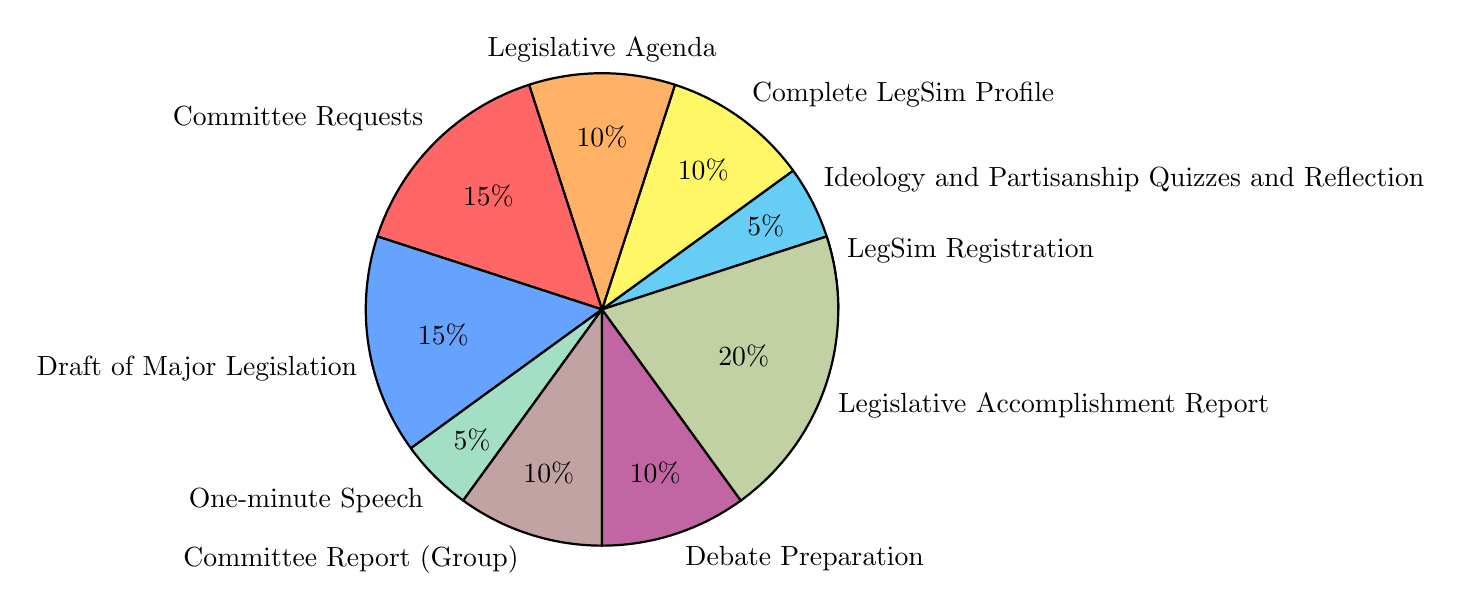
\begin{tikzpicture} 
		\pie{5/LegSim Registration, 5/Ideology and Partisanship Quizzes and Reflection, 10/Complete LegSim Profile, 10/Legislative Agenda, 15/Committee Requests, 15/Draft of Major Legislation, 5/One-minute Speech, 10/Committee Report (Group), 10/Debate Preparation, 20/Legislative Accomplishment Report}
	\end{tikzpicture}	
\end{center}

The letter grades will be assigned according to these percentages:

\begin{center}
	\begin{tabular}{ l l l l l l l l l l}
		\toprule
 		A+ & 97-100\% & B+ & 87-89\% & C+ & 77-79\% & D+ & 67-69\% & F & 0-59\% \\
		A & 93-96\% & B & 83-86\% & C & 73-76\% & D & 63-66\% \\
		A- & 90-92\% & B- & 80-82\% & C- & 70-72\% & D- & 60-62\% \\
		\bottomrule    
	\end{tabular}
\end{center}


\section*{Classroom Decorum and Academic Discourse}

Successful policy thrives on constructive and respectful disagreement. One of our most important goals is to create a classroom environment that supports respectful, critical inquiry through the free exchange of ideas. As part of learning, it is essential to discuss topics with individual who have different viewpoints than your own and the only way we can better understand one another is if we can carry on a collegial discussion of the topic. Remember, the goal is to become better critical thinkers. To do so we must learn to listen to others and articulate our views in respectful ways. As such, the following principles will guide our discussions and simulations:

\begin{itemize}
\item Treat every member of the class with respect, even if you disagree with their opinion;
\item Bring light, not heat;
\item Reasonable minds can differ on any number of perspectives, opinions, and conclusions;
\item Because constructive disagreement sharpens thinking, deepens understanding, and reveals novel insights, it is not just encouraged, it is expected;
\item No ideas are immune from scrutiny and debate;
\item You will not be graded on your opinions;
\item Arguments and evidence should be judged \emph{independently} of who offers such arguments and evidence. 
\end{itemize}

Additionally, to build a classroom environment that maximizes everyone's ability to master the course material please be mindful to not distract your fellow learners with your phone, tablet, or computer. It's perfectly fine if you would like to use these devices to take notes during class, but don't use them to distract yourself or your peers! Similarly, if you come late (or must leave early) please to enter/depart  the classroom in the least disruptive manner possible. This includes sitting near the door if you anticipate leaving early or taking a seat as near to the door as possible if you arrive late. 


\section*{Academic Honesty}

I expect that all work you produce for this course will be your own. If you plagiarize any material from outside sources for your written work or presentation in this course, or on the final exam, \textbf{it will result in a failure of the entire course.} There are no exceptions to this, and no second chances. Please refer to the university's \href{https://conduct.ucr.edu/policies/academic-integrity-policies-and-procedures}{Academic Integrity Polices \& Procedures} if you have questions about these standards. 


\section*{Special Accommodations}

If you need particular accommodations to help you succeed in mastering this course's material, please contact the \href{https://sdrc.ucr.edu}{Student Disability Resource Center} on campus in Costo Hall 125 to get a personalized accommodation plan.


\section*{Course Outline}

This syllabus is a working document and I may need to make changes to accommodate our simulations. I reserve the right to make changes to the assigned readings (additions or deletions) or to the order of topics we cover as I deem necessary. Announcements regarding schedule changes will be made in class, in discussion sections, or on iLearn.

Also note that this schedule lists the topics of discussion for each class. To master the course material, you should finish each meeting's readings before we discuss them in class. This schedule also indicates which course promise(s) each class contributes to. They are listed as \textbf{CP} followed by the specific promise's number (listed above). 

\paragraph*{Tentative Schedule:}
\begin{center}
\begin{calendar}{8/31/2020}{16} % Semester starts on 1/11/2010 and last for 12
                    % weeks, including finals week
\setlength{\calboxdepth}{.3in}
\MWClass
% schedule
\caltexton{1}{\textbf{CP 1} \\ Course Introduction; Overview of LegSim}
\caltextnext{\textbf{CP 1} \\ Congress and Its Members Ch. 1: What exactly is Congress and what do members do?}
\caltextnext{\textbf{CP 1} \\ {\color{red} Register for LegSim by Sep. 11th} \\ Congress and Its Members Ch. 2: How is Congress organized?}
\caltextnext{\textbf{CP 3} \\ {\color{red} Ideology and Partisanship Quizzes + Reflection Due} \\ Congress and Its Members Ch. 3 S. 1 \& 2: You gotta know the rules before you play (Campaign and election procedures).}
\caltextnext{\textbf{CP 1} \\ Congress and Its Members Ch. 3 S. 3-5: Entering the electoral race.}
\caltextnext{\textbf{CP 1 \& 3} \\ Congress and Its Members Ch. 4 S. 1-4: How to win!}
\caltextnext{\textbf{CP 1 \& 3} \\ Congress and Its Members Ch. 4 S. 5-8: What candidates need to know about voters.}
\caltextnext{\textbf{CP 1, 2, \& 3} \\ \textbf{Simulation Exercise:} Selecting your district. \\ Congress and Its Members Ch. 5: What do legislators really care about? You better be a people person and love traveling!}
\caltextnext{\textbf{CP 1, 2, \& 4} \\  {\color{red} Select Your Party and Complete LegSim Profile due Sep. 25th.} \\ Congress and Its Members Ch. 6 S. 1-4: Getting to know the bosses (leadership positions in Congress).}
\caltextnext{\textbf{CP 1, 2, \& 4} \\  \textbf{Simulation Exercise:} Party Meetings, Introductions, and Decide Leadership Positions \\ Congress and Its Members Ch. 6 S. 5-9: Supporting your team and joining clubs (Party committees and caucuses).}
\caltextnext{\textbf{CP 1} \\ Congress and Its Members Ch. 7 S. 1-4: Learn how things get done around here (committees). }
\caltextnext{\textbf{CP 1, 3, \& 4} \\ \textbf{Simulation Exercise:} Parties Meet to Elect Leaders \\ Congress and Its Members Ch. 7 S. 5-9: What happens after a bill gets introduced?}
\caltextnext{\textbf{CP 1 \& 2} \\ {\color{red} Finalize Your Legislative Agenda due Oct. 16th} \\ Congress and Its Members Ch. 8 S. 1-4: The House has a lot of rules.}
\caltextnext{\textbf{CP 1 \& 2} \\ Congress and Its Members Ch. 8 S. 5-8: So does the Senate... }
\caltextnext{\textbf{CP 1 \& 2} \\ Congress and Its Members Ch. 9 S. 1-2: What exactly do you do in Congress?}
\caltextnext{\textbf{CP 1} \\ {\color{red} Submit Committee Requests due Oct. 27th} \\ Congress and Its Members Ch. 9 S. 3-5: How much freedom do members have in Congress?}
\caltextnext{\textbf{CP 1 \& 4} \\ \textbf{Simulation Exercise:} Party Leaders meet to determine committee assignments. \\ Bill-writing workshop and procedural practice.}
\caltextnext{\textbf{CP 1} \\ Congress and Its Members Ch. 10 S. 1-2: Can the president really affect legislation?}
\caltextnext{\textbf{CP 1, 3, \& 4} \\ Congress and Its Members Ch. 10 S. 3-5: How the president can stifle all your hard work.}
\caltextnext{\textbf{CP 1 \& 4} \\ \textbf{Simulation Exercise:} The House convenes for the first time, members are sworn in, organizing resolutions are adopted, Speaker is elected, party and committee meetings.}
\caltextnext{\textbf{CP 1, 2, \& 4} \\ {\color{red} Submit your major piece of legislation due Nov. 15th} \\Congress and Its Members Ch. 13 Where do organized interests come in? Does money matter more than constituents?}
\caltextnext{\textbf{CP 1, 2 \& 4} \\ \textbf{Simulation Exercise:} Leaders determine how time will be allocated between committee meetings, party meetings, and speeches.}
\caltextnext{\textbf{CP 1, 2, \& 4} \\ \textbf{Simulation Exercise:} Committees meet during allocated time to discuss legislation.}
\caltextnext{\textbf{CP 1, 2, \&4} \\ {\color{red} Submit your debate preparation} \\\textbf{Simulation Exercise:} Parties meet to discuss legislative goals; committees meet to vote on legislation and write bill reports.}
\caltextnext{\textbf{CP 1, 2, \& 4} \\ \textbf{Simulation Exercise:} The House convenes to debate bills reported from committee.}
\caltextnext{\textbf{CP 1, 2, \& 4} \\ \textbf{Simulation Exercise:} The House continues debate and votes on bills.}
\caltextnext{\textbf{CP 1, 2, 3, \& 4} \\ Simulation Debrief}
\caltextnext{}
\caltextnext{\textbf{CP 2 \& 3} \\ {\color{red} Legislative Accomplishment Report Due}}
% ... and so on

% Holidays
\Holiday{9/7/2020}{\textbf{Labor Day - No Class :(}}
\Holiday{11/23/2020}{\textbf{Thanksgiving Break! - No Class :(}}
\Holiday{11/24/2020}{\textbf{Thanksgiving Break! - No Class :(}}
\Holiday{11/25/2020}{\textbf{Thanksgiving Break! - No Class :(}}
\Holiday{11/26/2020}{\textbf{Thanksgiving Break! - No Class :(}}
\Holiday{11/27/2020}{\textbf{Thanksgiving Break! - No Class :(}}
\Holiday{11/28/2020}{\textbf{Thanksgiving Break! - No Class :(}}
% ... and so on

\options{4/26/2010}{\noclassday} % finals week
\options{4/27/2010}{\noclassday} % finals week
\options{4/28/2010}{\noclassday} % finals week
\options{4/29/2010}{\noclassday} % finals week
\options{4/30/2010}{\noclassday} % finals week
\caltext{4/27/2010}{\textbf{Final Exam}}
\end{calendar}
\end{center}

\end{document}